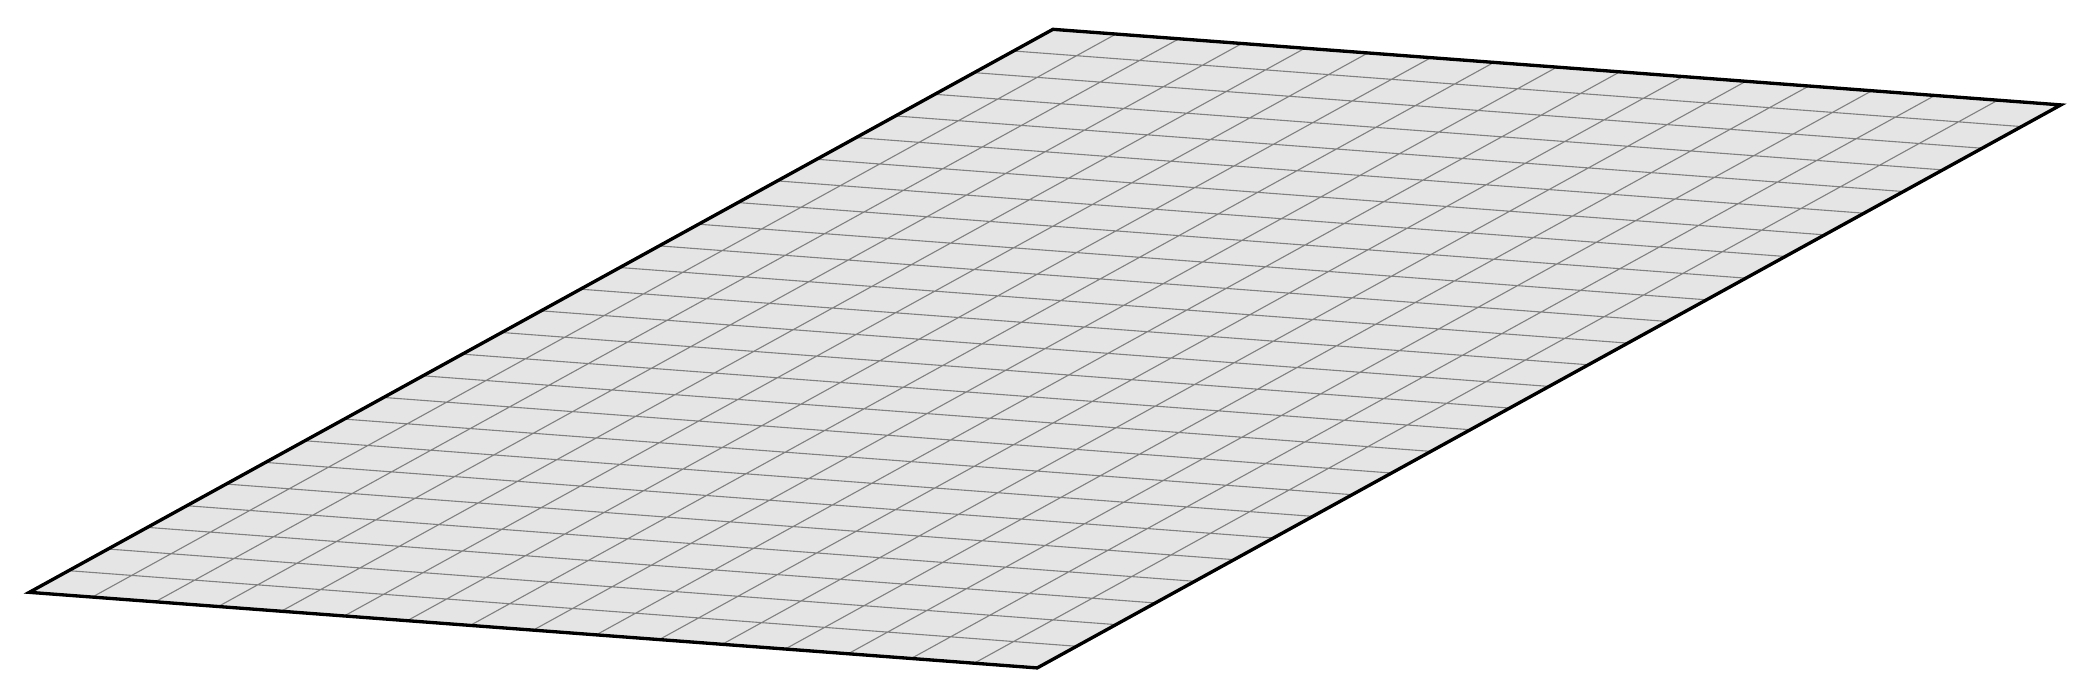
\begin{tikzpicture}
\def\h{80}% horizontaql viewing angle
\def\v{10}% vertical viewing angle
\begin{scope}[yshift=-180,yslant=.55,xslant=-1.6]
    %the rectangular surface onto which the clusters are located
    \filldraw[black!10,very thick] (0,1) rectangle (13,9);
    %circle circumventing the smallest cluster 
    \draw[step=5mm, thin, gray] (0,1) grid (13,9); %defining grids
    \draw[black,very thick] (0,1) rectangle (13,9);%marking borders    
    %\node[circle,circular glow,fill=gray!20,draw=gray,thick]
    %at (4.1,4.9) {\phantom{perimetro}};
\end{scope}
\end{tikzpicture}